\chapter{Biologi Kanker}\label{ch:b3:cancer-biology}

Sebuah \omterm{def:b3:cancer-biology:hallmarks}{tumor} yang cukup besar untuk teraba, yakni satu sentimeter lebarnya,
memuat semiliar sel dan merupakan hasil kira-kira tiga puluh pelipatduaan dari
satu sel yang menyimpang --- lazimnya sedasawarsa pertumbuhan sebelum siapa pun
mengetahuinya. Di balik sel itu terdapat beberapa mutasi, dan masing-masing
harus terjadi pada garis keturunan yang sama serta masing-masing membuang satu
kendali kedua bab sebelumnya: sebuah rem pada pembelahan, sebuah pemicu
kematian, sebuah batas pada cacah pembelahan, sebuah tuntutan untuk tinggal di
tempat. \omterm{def:b3:cancer-biology:hallmarks}{Kanker} adalah evolusi sebuah populasi sel di dalam sebuah tubuh, lewat
mutasi dan seleksi, menuju keadaan yang melayani selnya lalu membunuh
organismenya. Bab ini membahas gen yang terkena dan apa yang biasanya
dikerjakannya, statistika yang menyingkapkan berapa pukulan yang dibutuhkan,
fisiologi yang harus diperoleh sebuah \omterm{def:b3:cancer-biology:hallmarks}{tumor} agar tumbuh melampaui satu
milimeter dan agar menyebar, penyebab yang dapat dihindari, serta terapinya ---
dari racun yang membunuh sel yang membelah sampai antibodi yang melepaskan
sistem kekebalan --- yang dimungkinkan biologinya, beserta alasan evolusi
mengapa terapi itu begitu sering gagal.

\section{Apa itu kanker}

\begin{definition}[Tumor, kanker, ciri khasnya]\label{def:b3:cancer-biology:hallmarks}
\index{kanker}\index{tumor}\index{ganas}\index{metastasis}\index{ciri khas kanker}
Sebuah \emph{tumor} (neoplasma) adalah klon sel yang telah lolos dari
kendali atas pertumbuhannya lalu menumpuk di dalam sebuah jaringan. Ia disebut
\emph{jinak} bila tetap terkurung dan terbungkus, dan disebut \emph{ganas} ---
yakni sebuah \emph{kanker} --- bila selnya menyerbu jaringan tetangganya lalu
menyemaikan tumor sekunder di tempat lain (\emph{metastasis}), dan itulah yang
membunuh. Kanker dinamai menurut sel asalnya: karsinoma dari epitelium
(\qty{85}{\%} kanker manusia), sarkoma dari jaringan ikat,
leukemia dan limfoma dari sel pembentuk darah, glioma dari glia.
Pada jaringan apa pun, sebuah klon yang ganas telah memperoleh perangkat
kemampuan yang sama, yakni \emph{ciri khas kanker}: ia berproliferasi tanpa
isyarat pertumbuhan dari luar lalu mengabaikan isyarat yang akan
menghentikannya; ia menahan \omterm{def:b3:cell-cycle-apoptosis:apoptosis}{apoptosis}; ia membelah tanpa batas karena telah
mengaktifkan kembali \omterm{def:b3:cancer-biology:telomerase}{telomerase}; ia mengimbas pembuluh darah; ia menyerbu lalu
bermetastasis; dan, yang mendasari semuanya, genomnya tak mantap, ia
memprogram ulang metabolismenya ke arah glikolisis bahkan dalam oksigen (efek
Warburg), ia merekrut sel radang yang membantunya, dan ia mengelak dari sistem
kekebalan. Tiap ciri khasnya adalah sebuah kendali jaringan normal yang
dikalahkan, dan masing-masing terpetakan pada gen.
\end{definition}

\begin{omfigure}
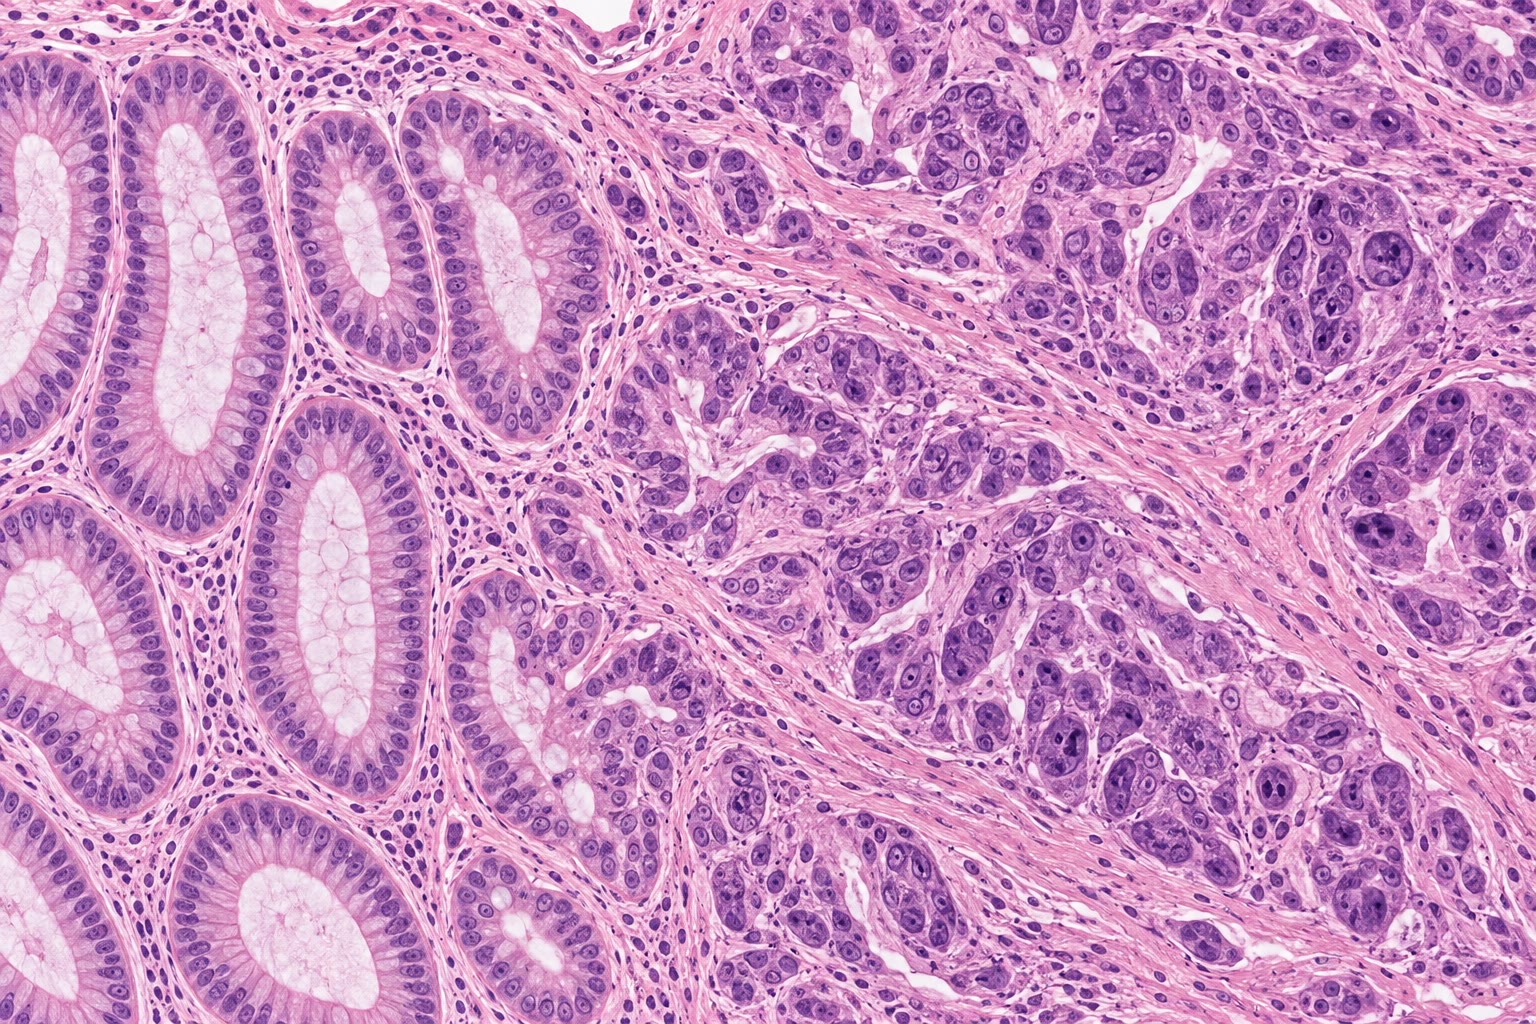
\includegraphics[width=0.56\linewidth]{images/book5/ai/b5-11-tumour-histology.jpg}

{\small Sebuah karsinoma pada batasnya: di sebelah kiri, epitelium kelenjar
yang tertib dengan nukleus yang teratur; di sebelah kanan, sel yang berjejal
dengan nukleus yang besar dan tak teratur yang menyerbu stroma di bawahnya ---
yakni gambaran yang dibaca seorang patolog untuk menyebut sebuah \omterm{def:b3:cancer-biology:hallmarks}{tumor} \omterm{def:b3:cancer-biology:hallmarks}{ganas}.}
\end{omfigure}

\section{Gen yang terkena}

\begin{definition}[Onkogen dan penekan tumor]\label{def:b3:cancer-biology:genes}
\index{onkogen}\index{protoonkogen}\index{gen penekan tumor}%
\index{Ras}\index{p53}\index{hipotesis dua pukulan}
Sebuah \emph{protoonkogen} adalah gen normal yang memacu proliferasi atau
ketahanan hidup --- sebuah faktor pertumbuhan, reseptornya, sebuah protein
pengisyarat, sebuah faktor transkripsi, sebuah \omterm{def:b3:cell-cycle-apoptosis:cdk}{siklin} --- dan sebuah
\emph{onkogen} adalah bentuk mutannya yang aktif tanpa isyarat normalnya:
sebuah mutasi titik yang mengunci \omterm{def:b3:membrane-traffic:coats}{GTPase kecil} \emph{Ras} pada keadaan GTP-nya
(glisina~12 pada seperempat seluruh \omterm{def:b3:cancer-biology:hallmarks}{kanker}), sebuah penguatan gen reseptor
HER2 atau gen faktor transkripsi Myc, sebuah translokasi yang memfusikan
\emph{BCR} pada kinase \emph{ABL} pada leukemia mieloid menahun atau yang
menaruh \emph{MYC} di samping sebuah penguat antibodi pada limfoma Burkitt.
Satu alel mutan sudah memadai: onkogen bekerja secara dominan. Sebuah
\emph{gen penekan \omterm{def:b3:cancer-biology:hallmarks}{tumor}} mengekang proliferasi atau memaksakan kematian
maupun perbaikan --- Rb dan p16 pada \omterm{def:b3:cell-cycle-apoptosis:checkpoints}{titik batasnya}, \emph{p53}, yakni penjaga
yang menghentikan atau membunuh sel yang rusak, APC pada \omterm{prop:b3:cancer-biology:pathways}{jalur Wnt} usus besar,
PTEN, BRCA1 dan BRCA2, serta gen \omterm{prop:b3:dna-repair:fidelity}{perbaikan salah pasang} --- dan gen itu harus
kehilangan kedua alelnya agar menyumbang: \emph{dua pukulan}, dan yang pertama
kerap diwarisi pada sindrom \omterm{def:b3:cancer-biology:hallmarks}{kanker} keluarga, sedangkan yang kedua somatik.
\emph{p53} termutasi pada separuh seluruh \omterm{def:b3:cancer-biology:hallmarks}{kanker} manusia dan jalurnya
dilumpuhkan pada sebagian besar sisanya.
\end{definition}

\begin{proof}[Bukti eksperimental]
Rous (1911) menularkan sarkoma ayam dengan filtrat bebas sel, yakni
sebuah virus, yang gen pengubahnya yang tunggal, \emph{src}, ditunjukkan
Varmus dan Bishop (1976) sebagai salinan tangkapan sebuah gen ayam yang normal
--- \omterm{def:b3:cancer-biology:genes}{onkogen} adalah gen sel yang berubah. Weinberg (1982) memindahkan
DNA dari karsinoma kandung kemih manusia ke dalam sel mencit biakan, yang lalu
berubah; fragmen yang bertanggung jawab adalah \emph{RAS} dengan
satu perubahan basa, dan perubahan yang sama tak ada pada jaringan normal
pasiennya. Knudson (1971) membandingkan anak yang mengidap \omterm{def:b3:cancer-biology:hallmarks}{tumor} mata
bernama retinoblastoma: yang memiliki riwayat keluarga mengembangkan beberapa
\omterm{def:b3:cancer-biology:hallmarks}{tumor} pada kedua matanya, sejak dini; yang tidak memilikinya mengembangkan
satu \omterm{def:b3:cancer-biology:hallmarks}{tumor}, lebih lambat --- yang selaras dengan kasus keluarganya menuntut
satu peristiwa somatik dan kasus sporadisnya dua, dan karena itu selaras
dengan sebuah gen yang kedua salinannya harus hilang. \emph{RB} diklon
pada tahun 1986 dan kedua alelnya memang dilumpuhkan pada tiap \omterm{def:b3:cancer-biology:hallmarks}{tumornya}.
\end{proof}

\begin{theorem}[Pukulan dan kurva umurnya]\label{thm:b3:cancer-biology:armitage-doll}
\index{model Armitage--Doll}\index{karsinogenesis bertahap}
Andaikan sebuah \omterm{def:b3:cancer-biology:hallmarks}{kanker} menuntut $k$ peristiwa bebas yang membatasi laju pada
satu garis keturunan sel, dan masing-masing terjadi dengan laju tetap $u$ tiap
sel tiap tahun, di dalam populasi $N$ sel yang rentan, dengan $ut \ll 1$. Maka
peluang bahwa sebuah sel tertentu telah mengalami seluruh $k$ peristiwa itu
pada umur $t$ kira-kira $(ut)^{k}$, risiko kumulatif jaringannya kira-kira
$N(ut)^{k}$, dan insidensinya --- yakni kasus baru tiap tahun pada umur $t$ ---
\[
I(t) \approx N\,k\,u^{k}\,t^{\,k-1},
\]
yakni sebuah pangkat umur dengan eksponen $k - 1$: sebuah garis lurus
berkemiringan $k - 1$ pada plot log--log. Bagi seorang yang mewarisi salah satu
peristiwanya, \omterm{def:b3:cancer-biology:hallmarks}{kanker} yang sama berinsidensi $\propto t^{\,k-2}$, yakni satu
pangkat lebih rendah.
\end{theorem}
\begin{proof}
Tiap peristiwanya, yang berlaju $u$, telah terjadi pada waktu $t$ dengan
peluang $1 - e^{-ut} \approx ut$; peristiwanya saling bebas, sehingga seluruh
$k$ peristiwa telah terjadi dengan peluang $(ut)^{k}$, dan urutan terjadinya
tak berarti di sini. Dengan $N$ sel dan peristiwa yang langka, harapan cacah
sel yang telah merampungkan runtunannya adalah
$N(ut)^{k}$, dan insidensinya adalah turunan waktunya, $Nku^{k}t^{k-1}$.
Mewarisi satu peristiwa menyisakan $k - 1$ peristiwa: $(ut)^{k-1}$, dengan
insidensi $\propto t^{k-2}$. Andaikan urutan peristiwanya berarti (hanya $1$
dari $k!$ urutan yang menuju \omterm{def:b3:cancer-biology:hallmarks}{kanker}), prafaktornya yang berubah, bukan eksponennya.
\end{proof}

\begin{example}[Membaca eksponennya]\label{ex:b3:cancer-biology:exponent}
Insidensi sebagian besar karsinoma pada orang dewasa naik kira-kira sebagai
pangkat kelima sampai keenam umurnya --- dari kira-kira $1$ dari \num{100000}
tiap tahun pada umur tiga puluh menjadi $1$ dari $300$ pada umur delapan
puluh, yakni faktor $300$ bagi faktor $2.7$ pada umurnya, dan
$2.7^{5.7} \approx 300$ --- yang menyarankan enam atau tujuh peristiwa
pembatas laju. Taksirannya kasar: mengembangnya sebuah klon sesudah tiap
pukulan menaikkan cacah sel yang berisiko terkena pukulan berikutnya,
sehingga lebih sedikit peristiwa dengan pertumbuhan klonal di antaranya memberi
kemiringan yang sama, dan cacah mutasi \emph{pemacu} yang ditemukan pada \omterm{def:b3:cancer-biology:hallmarks}{tumor}
yang telah diurutkan adalah dua sampai delapan. Retinoblastoma Knudson cocok
persis dengan pernyataan kedua teoremanya: penyakit sporadisnya, yang menuntut
dua pukulan, berinsidensi yang naik dengan umur (sepanjang beberapa tahun
retinoblasnya ada); penyakit turunannya, yang menuntut satu, hadir pada laju
yang nyaris tetap sejak lahir lalu menyerang dini dan berulang kali.
\end{example}

\begin{omfigure}
\begin{tikzpicture}
\begin{axis}[
  width=0.68\linewidth, height=6cm,
  xmode=log, ymode=log,
  xmin=20, xmax=100, ymin=1e-6, ymax=1e-1,
  xlabel={umur (tahun)}, ylabel={insidensi tiap orang tiap tahun},
  xlabel style={font=\small, at={(axis description cs:0.5,-0.12)}, anchor=north},
  ylabel style={font=\small},
  tick label style={font=\small}, xtick={20,30,50,80}, xticklabels={20,30,50,80},
  clip=false,
]
\addplot[very thick, omThm, domain=20:100, samples=2] {1e-5*(x/30)^5.7};
\addplot[very thick, omDef, domain=20:100, samples=2] {3e-4*(x/30)^1};
\addplot[very thick, omMeth!70!black, domain=20:100, samples=2] {2e-3};
\node[font=\scriptsize, omThm, anchor=south west] at (axis cs:38,2.5e-6) {karsinoma: kemiringan $5$--$6$, enam atau tujuh peristiwa};
\node[font=\scriptsize, omDef, anchor=south west] at (axis cs:22,6e-4) {dua pukulan: kemiringan 1};
\node[font=\scriptsize, omMeth!70!black, anchor=south west] at (axis cs:22,2.3e-3) {satu pukulan diwarisi: kemiringan 0};
\end{axis}
\end{tikzpicture}

{\small Insidensi terhadap umur pada sumbu logaritmik. Sebuah \omterm{def:b3:cancer-biology:hallmarks}{kanker} yang
menuntut $k$ peristiwa pembatas laju naik sebagai $t^{k-1}$: garis curam
karsinoma dewasa, dan kedua kasus Knudson --- sebuah \omterm{def:b3:cancer-biology:hallmarks}{tumor} dua pukulan yang
naik secara lurus, dan \omterm{def:b3:cancer-biology:hallmarks}{tumor} yang sama pada pembawa satu pukulan warisan,
pada laju yang tetap sejak lahir.}
\end{omfigure}

\begin{proposition}[Jalur yang terkena]\label{prop:b3:cancer-biology:pathways}
\index{jalur Ras--MAPK}\index{jalur PI3K}\index{jalur Wnt}
Ratusan gen \omterm{def:b3:cancer-biology:hallmarks}{kanker} itu terbagi ke dalam selusin jalur, dan tiap jalurnya
dilumpuhkan sebuah \omterm{def:b3:cancer-biology:hallmarks}{tumor} pada satu titik. Jalur faktor pertumbuhannya: sebuah
kinase tirosina reseptor (EGFR, HER2), lalu \omterm{def:b3:cancer-biology:genes}{Ras}, lalu riam kinase
Raf--MEK--ERK menuju nukleusnya, dan sejajar dengannya PI3K--Akt--mTOR menuju ketahanan hidup dan
pertumbuhan, yang dikekang PTEN; sebuah \omterm{def:b3:cancer-biology:hallmarks}{tumor} mengaktifkan salah satunya, lewat
gen mana pun. Rem \omterm{def:b3:cell-cycle-apoptosis:cdk}{daur selnya}: \omterm{def:b3:cell-cycle-apoptosis:cdk}{siklin} D, Cdk4, p16, Rb (\cref{ch:b3:cell-cycle-apoptosis}).
Penjaganya: \omterm{def:b3:cancer-biology:genes}{p53} dan pengaturnya. Kematiannya: Bcl-2. Pengisyaratan
perkembangan: Wnt (APC, $\beta$-katenin) di usus besar, Hedgehog di kulit
dan otak, Notch di sel~T. Pemeliharaan genomnya: \omterm{prop:b3:dna-repair:fidelity}{perbaikan salah pasang},
\omterm{def:b3:dna-repair:dsb}{BRCA}, \omterm{def:b3:dna-repair:ddr}{ATM}. \omterm{def:b3:chromatin-epigenetics:nucleosome}{Kromatinnya}: \omterm{def:b3:chromatin-epigenetics:histone-code}{penulis} dan penata ulang
\cref{ch:b3:chromatin-epigenetics}, yang termutasi pada sepertiga \omterm{def:b3:cancer-biology:hallmarks}{tumor}.
Kebakaannya: promotor \omterm{def:b3:cancer-biology:telomerase}{telomerase}. Karena sebuah jalur adalah runtunan
langkah, mutasi pada gen yang berbeda menjadi alternatif --- sebuah \omterm{def:b3:cancer-biology:hallmarks}{tumor}
\omterm{def:b3:cancer-biology:genes}{ber-Ras} mutan jarang pula ber-EGFR mutan --- dan obat melawan satu langkahnya
dapat dikalahkan sebuah mutasi di hilirnya.
\end{proposition}

\begin{omfigure}
\begin{tikzpicture}[every node/.style={font=\scriptsize}, >=stealth]
  % membrane
  \draw[very thick, omDef] (0,3.6) -- (12,3.6); \draw[very thick, omDef] (0,3.3) -- (12,3.3);
  \node[above] at (1.0,3.65) {luar}; \node[below] at (1.0,3.25) {sitosol};
  % receptor
  \draw[thick, fill=omProp!35] (3.7,3.0) rectangle (4.1,4.1); \draw[thick, fill=omProp!35] (4.3,3.0) rectangle (4.7,4.1);
  \node[above, align=center] at (4.2,4.15) {faktor pertumbuhan $\to$ kinase reseptor\\(EGFR, HER2)}; \node[right, omThm, font=\tiny] at (4.75,4.0) {diperkuat};
  % Ras
  \node[draw, thick, rounded corners, fill=omDef!20] (ras) at (4.2,2.3) {Ras--GTP};
  \node[right, omThm, font=\tiny] at (5.0,2.3) {G12: selalu menyala};
  \node[draw, thick, rounded corners, fill=omDef!20] (raf) at (4.2,1.4) {Raf $\to$ MEK $\to$ ERK};
  \node[right, omThm, font=\tiny] at (5.8,1.4) {BRAF V600E};
  \node[draw, thick, rounded corners, fill=omMeth!25] (myc) at (4.2,0.4) {Myc, siklin D: proliferasi};
  \node[right, omThm, font=\tiny] at (6.4,0.4) {Myc diperkuat};
  \draw[->, thick] (4.2,3.0) -- (ras); \draw[->, thick] (ras) -- (raf); \draw[->, thick] (raf) -- (myc);
  % PI3K branch
  \node[draw, thick, rounded corners, fill=omDef!20] (pi3k) at (9.6,2.3) {PI3K $\to$ Akt $\to$ mTOR};
  \node[draw, thick, rounded corners, fill=omMeth!25] (surv) at (9.6,0.4) {ketahanan hidup, pertumbuhan};
  \draw[->, thick] (4.7,3.0) .. controls (6.5,2.8) .. (pi3k.north west); \draw[->, thick] (pi3k) -- (surv);
  \node[draw, thick, rounded corners, fill=omThm!15] (pten) at (12.2,1.4) {PTEN}; \draw[-|, thick, omThm] (pten) -- (9.6,1.4);
  \node[below, omThm, font=\tiny] at (12.2,1.15) {terhapus};
  % p53 and Rb on the side
  \node[draw, thick, rounded corners, fill=omThm!15] (rb) at (1.2,0.4) {Rb, p16}; \draw[-|, thick, omThm] (rb) -- (myc);
  \node[below, omThm, font=\tiny, align=center] at (1.2,0.15) {kedua alelnya hilang};
  \node[draw, thick, rounded corners, fill=omThm!15] (p53) at (1.2,1.6) {p53}; \node[below, omThm, font=\tiny, align=center] at (1.2,1.35) {termutasi pada separuh\\kanker};
  \draw[-|, thick, omThm] (p53) -- (1.2,0.65);
\end{tikzpicture}

{\small Jalur faktor pertumbuhannya dan tempat \omterm{def:b3:cancer-biology:hallmarks}{kanker} memukulnya. Kotak
hijaunya adalah keluarannya, kotak birunya langkah pengisyaratan yang dikunci
mutasi onkogenik, dan kotak merahnya penekan yang hilang dari \omterm{def:b3:cancer-biology:hallmarks}{tumor} (batangnya
menandai penghambatan). Sebuah \omterm{def:b3:cancer-biology:hallmarks}{tumor} lazimnya mengusung satu cacat pengaktif
dan satu atau dua cacat pelumpuh pada diagram ini.}
\end{omfigure}

\section{Sebuah tumor berevolusi}

\begin{proposition}[Karsinogenesis bertahap]\label{prop:b3:cancer-biology:multistep}
\index{mutasi pemacu}\index{mutasi penumpang}%
\index{evolusi klonal}\index{tanda tangan mutasi}
Sebuah \omterm{def:b3:cancer-biology:hallmarks}{tumor} adalah hasil evolusi somatik: mutasi menghasilkan
varian, dan seleksi di dalam jaringannya memihak varian yang membelah lebih
banyak, mati lebih sedikit, atau lolos dari sebuah kekangan. Runtunan
kolorektal yang dipecahkan Vogelstein menjadi paradigmanya: hilangnya
\emph{APC} menghasilkan sebuah polip jinak yang kecil; sebuah mutasi
\emph{KRAS} membiarkannya tumbuh menjadi sebuah adenoma; hilangnya
\emph{SMAD4} atau \emph{TP53} mengubahnya menjadi karsinoma; perubahan
selanjutnya memungkinkan \omterm{def:b3:cancer-biology:metastasis}{invasi}. Tiap langkahnya adalah pengembangan klonal
yang melipatgandakan sel yang berisiko terkena langkah berikutnya. Sebuah
\omterm{def:b3:cancer-biology:hallmarks}{tumor} yang telah diurutkan mengusung ribuan mutasi, dan segelintir di
antaranya --- lazimnya dua sampai delapan --- menjadi \emph{pemacu} yang
memberi keunggulan terpilih; sisanya \emph{penumpang}, yang terbawa di dalam
klonnya, dan jangkauannya menjadi catatan tentang apa yang menyebabkannya:
C$\to$T pada pirimidina bersebelahan dari cahaya ultraungu pada melanoma,
G$\to$T dari asap tembakau pada \omterm{def:b3:cancer-biology:hallmarks}{kanker} paru-paru, sidik jari enzim APOBEC,
sidik jari \omterm{prop:b3:dna-repair:fidelity}{perbaikan salah pasang} yang cacat, sidik jari aflatoksin --- yakni
\emph{\omterm{prop:b3:cancer-biology:multistep}{tanda tangan mutasi}}. \omterm{def:b3:cancer-biology:hallmarks}{Tumor} bersifat heterogen, yakni sebuah pohon
subklon yang bercabang, dan subklon yang membunuh kerap merupakan minoritas
pada saat diagnosisnya.
\end{proposition}

\begin{omfigure}
\begin{tikzpicture}[every node/.style={font=\scriptsize}, >=stealth]
  \foreach \x/\lab/\gene/\col/\r in {0/epitelium normal/{}/omDef!20/0.5, 2.6/polip kecil/{APC hilang (kedua alel)}/omDef!35/0.7, 5.4/adenoma/{KRAS aktif}/omProp!40/1.0, 8.4/karsinoma/{SMAD4 atau TP53 hilang}/omThm!35/1.3, 11.6/{invasif, metastatik}/{pemacu lanjutan,\\ketakmantapan}/omThm!60/1.5} {
    \draw[thick, fill=\col] (\x,0) circle (\r);
    \node[below, align=center] at (\x,-1.6) {\lab};
    \node[above, align=center, omThm] at (\x,1.6) {\gene};
  }
  \foreach \a/\b in {0.5/1.9, 3.3/4.4, 6.4/7.1, 9.7/10.1} \draw[->, very thick] (\a,0) -- (\b,0);
  \node[below, align=center] at (5.8,-2.3) {sepuluh sampai tiga puluh tahun; tiap langkahnya pengembangan klonal\\yang melipatgandakan sel yang berisiko terkena langkah berikutnya};
\end{tikzpicture}

{\small Runtunan kolorektalnya. Tiap \omterm{prop:b3:cancer-biology:multistep}{mutasi pemacu} mengembangkan sebuah klon,
dan klon yang mengembang itu memasok sel yang di dalamnya pemacu berikutnya
dapat timbul; seluruh jalurnya memakan beberapa dasawarsa, dan itulah sebabnya
penapisan polip mencegah \omterm{def:b3:cancer-biology:hallmarks}{kankernya}.}
\end{omfigure}

\begin{method}[Uji Ames]\label{met:b3:cancer-biology:ames}
\index{uji Ames}\index{mutagen}
Untuk menguji apakah sebuah zat kimia bersifat mutagenik, dan karena itu
mungkin karsinogen: (1) ambillah galur \emph{Salmonella} dengan mutasi titik
pada sebuah gen biosintesis histidina, yang tak dapat tumbuh tanpa histidina;
(2) campurkanlah zat kimianya dengan ekstrak hati, yang enzimnya mengubah
banyak senyawa menjadi bentuk mutageniknya yang aktif, sebagaimana tubuh
melakukannya; (3) tebarkanlah sekitar $10^{8}$ bakteri pada agar bebas
histidina bersama campurannya; (4) hitunglah koloni yang tumbuh --- tiap koloni
adalah revertan yang sebuah mutasi baru telah memulihkan gennya; (5)
bandingkanlah dengan laju spontannya. Kenaikan revertan yang bergantung dosis
berarti senyawanya menimbulkan mutasi titik. Sebagian besar karsinogen yang
dikenal berhasil positif; ujinya murah, memakan dua hari, dan senyawa yang tak
lolos diperiksa lebih lanjut sebelum dibuat.
\end{method}

\begin{definition}[Kebakaan dan ketakmantapan]\label{def:b3:cancer-biology:telomerase}
\index{telomerase}\index{ketakmantapan kromosom}\index{aneuploidi!pada kanker}
Sel somatik yang normal tak memiliki telomerase lalu menghitung pembelahannya
lewat panjang telomernya (\cref{ch:b3:stem-cells}): sesudah kira-kira lima
puluh pembelahan sel itu menua, dan sel yang melewati \omterm{def:b3:cell-cycle-apoptosis:other}{penuaan sel} dengan
kehilangan \omterm{def:b3:cancer-biology:genes}{p53} dan Rb terus berjalan sampai telomernya terkuras lalu
kromosomnya berfusi dan patah --- yakni sebuah krisis yang membunuh sebagian
besar klonnya. Penyintas yang langka telah mengaktifkan kembali
\emph{telomerase}, biasanya lewat mutasi promotor, lalu menjadi baka;
\qty{90}{\%} \omterm{def:b3:cancer-biology:hallmarks}{kanker} mengekspresikan enzim itu. Krisisnya meninggalkan parut:
kromosom yang berfusi dan patah, penguatan, penghapusan, translokasi ---
yakni \emph{ketakmantapan kromosom}, yang, bersama hilangnya titik periksa
gelendong dan hilangnya tanggapan \omterm{def:b3:cancer-biology:genes}{p53} atas kesalahan pemilahan, membuat
sebagian besar \omterm{def:b3:cancer-biology:hallmarks}{tumor} padat menjadi aneuploid lalu menjaganya tetap
menghasilkan varian. Sebagian kecil \omterm{def:b3:cancer-biology:hallmarks}{tumor} justru berfenotipe mutator karena
hilangnya \omterm{prop:b3:dna-repair:fidelity}{perbaikan salah pasang}, dengan kariotipe normal dan laju mutasi
titik seribu kali lipat.
\end{definition}

\section{Tumor sebagai sebuah jaringan}

\begin{proposition}[Oksigen menetapkan ukuran tumor tanpa pembuluh]\label{prop:b3:cancer-biology:oxygen}
\index{angiogenesis}\index{batas difusi}\index{hipoksia}
Tinjaulah jaringan yang memakai oksigen dengan laju tetap $q$ tiap satuan
volume, yang dipasok lewat difusi (koefisiennya $D$) dari sebuah pembuluh yang
kepekatan pada dindingnya $c_{0}$. Dalam satu dimensi pada keadaan tunak, $D\,
\mathrm{d}^{2}c/\mathrm{d}x^{2} = q$, sehingga $c(x) = c_{0} - qx^{2}/2D$ dan
oksigennya habis pada jarak
\[
L = \sqrt{\frac{2Dc_{0}}{q}} .
\]
Dengan $D = \qty{2e-9}{m^2/s}$, $c_{0} = \qty{0.05}{mol/m^3}$, dan $q =
\qty{0.03}{mol/m^3/s}$ (sebuah \omterm{def:b3:cancer-biology:hallmarks}{tumor} yang bernapas), $L \approx \qty{80}{\micro
m}$: tak ada sel yang dapat hidup lebih dari kira-kira seratus mikrometer dari
sebuah kapiler. Sebuah klon tanpa pembuluh miliknya sendiri karena itu berhenti
pada garis tengah satu sampai dua milimeter, dengan pusatnya nekrotik dan
tepinya hidup. Untuk tumbuh lebih jauh ia harus mengimbas \emph{angiogenesis}
--- sel hipoksianya memantapkan faktor transkripsi HIF, yang mengimbas
VEGF, yang membuat sel endotelium terdekat bertunas ke arahnya. Judah
Folkman mengusulkan pada tahun 1971 bahwa menghalangi langkah itu akan
melaparkan \omterm{def:b3:cancer-biology:hallmarks}{tumornya}; antibodi melawan VEGF kini menjadi baku pada beberapa
\omterm{def:b3:cancer-biology:hallmarks}{kanker}, walaupun \omterm{def:b3:cancer-biology:hallmarks}{tumornya} menyesuaikan diri.
\end{proposition}
\begin{proof}
Pada keadaan tunak, fluks difusi $-D\,\mathrm{d}c/\mathrm{d}x$ harus
berubah terhadap $x$ tepat secepat oksigennya dipakai: $\mathrm{d}(-D\,
\mathrm{d}c/\mathrm{d}x)/\mathrm{d}x = -q$, yakni $D c'' = q$.
Mengintegralkannya dua kali dengan $c(0) = c_{0}$ dan $c'(L) = 0$ pada
kedalaman ketika tak ada lagi yang tersisa (tanpa fluks di seberangnya) memberi
$c = c_{0} - qx^{2}/2D$ sesudah memakai $c(L) = 0$ untuk menetapkan $L$.
Angkanya menyusul.
\end{proof}

\begin{omfigure}
\begin{tikzpicture}
\begin{axis}[
  width=0.6\linewidth, height=5.4cm,
  axis x line=bottom, axis y line=left,
  xmin=0, xmax=120, ymin=0, ymax=0.06,
  xlabel={jarak dari kapilernya ($\unit{\micro m}$)}, ylabel={oksigen ($\unit{mol/m^3}$)},
  xlabel style={font=\small, at={(axis description cs:0.5,-0.12)}, anchor=north},
  ylabel style={font=\small},
  tick label style={font=\small}, xtick={0,40,80,120}, ytick={0,0.025,0.05},
  clip=false,
]
\addplot[very thick, omDef, domain=0:81.6, samples=40] {0.05 - 0.03*(x*1e-6)^2/(2*2e-9)};
\addplot[very thick, omDef, domain=81.6:120, samples=2] {0};
\fill[omThm!25] (axis cs:81.6,0) rectangle (axis cs:120,0.06);
\node[font=\scriptsize, omThm!70!black, anchor=south, align=center] at (axis cs:100,0.03) {tanpa oksigen:\\nekrosis};
\node[font=\scriptsize, omDef, anchor=south west] at (axis cs:5,0.052) {$c(x) = c_{0} - qx^{2}/2D$};
\draw[dashed, gray] (axis cs:81.6,0) -- (axis cs:81.6,0.06); \node[font=\scriptsize, anchor=south west] at (axis cs:83,0.002) {$L$};
\end{axis}
\end{tikzpicture}

{\small Oksigen di dalam jaringan yang bernapas turun sebagai parabola
terhadap jarak dari kapiler terdekatnya lalu terkuras pada
$L = \sqrt{2Dc_{0}/q}$, yakni kira-kira \qty{80}{\micro m} di sini. Sebuah
\omterm{def:b3:cancer-biology:hallmarks}{tumor} tanpa pembuluh adalah cangkang sel hidup setebal itu yang mengelilingi
sebuah inti yang mati.}
\end{omfigure}

\begin{omfigure}
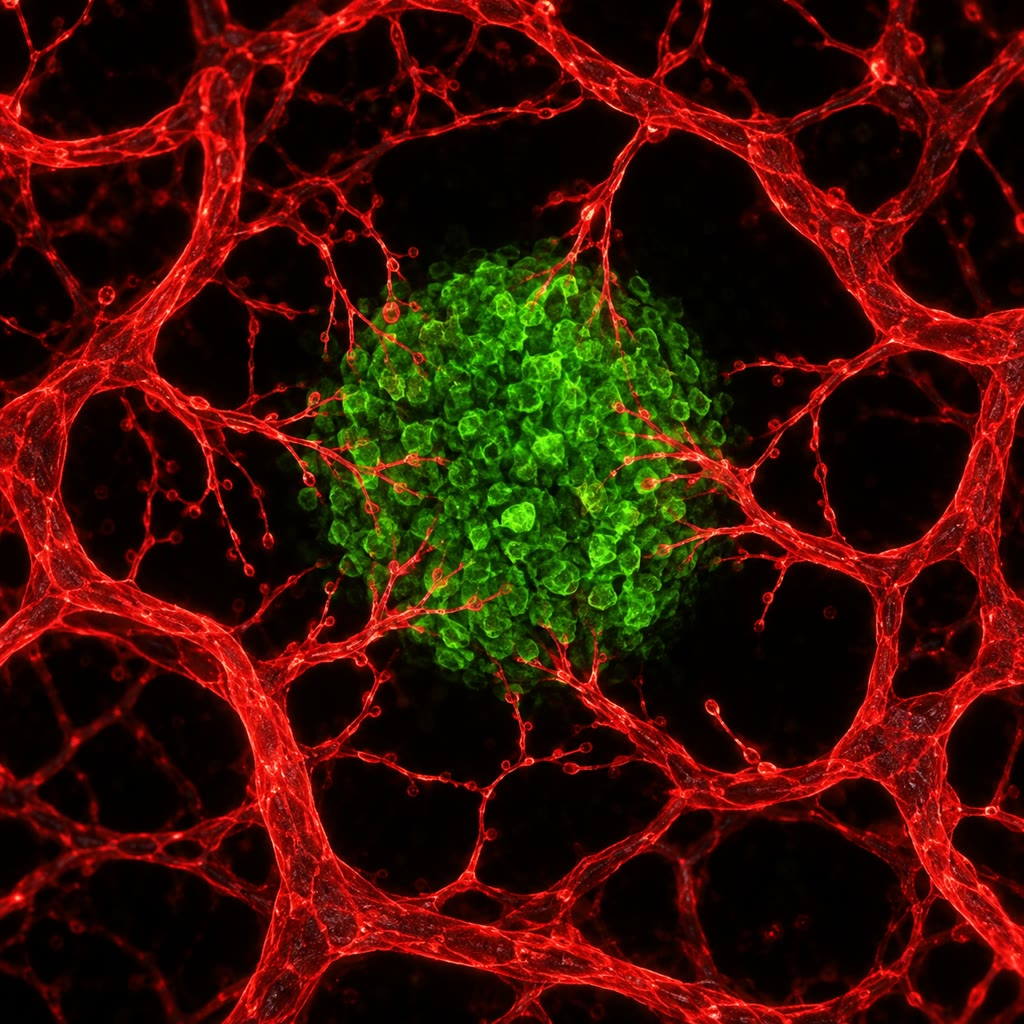
\includegraphics[width=0.36\linewidth]{images/book5/ai/b5-11-angiogenesis.jpg}\hspace{0.04\linewidth}
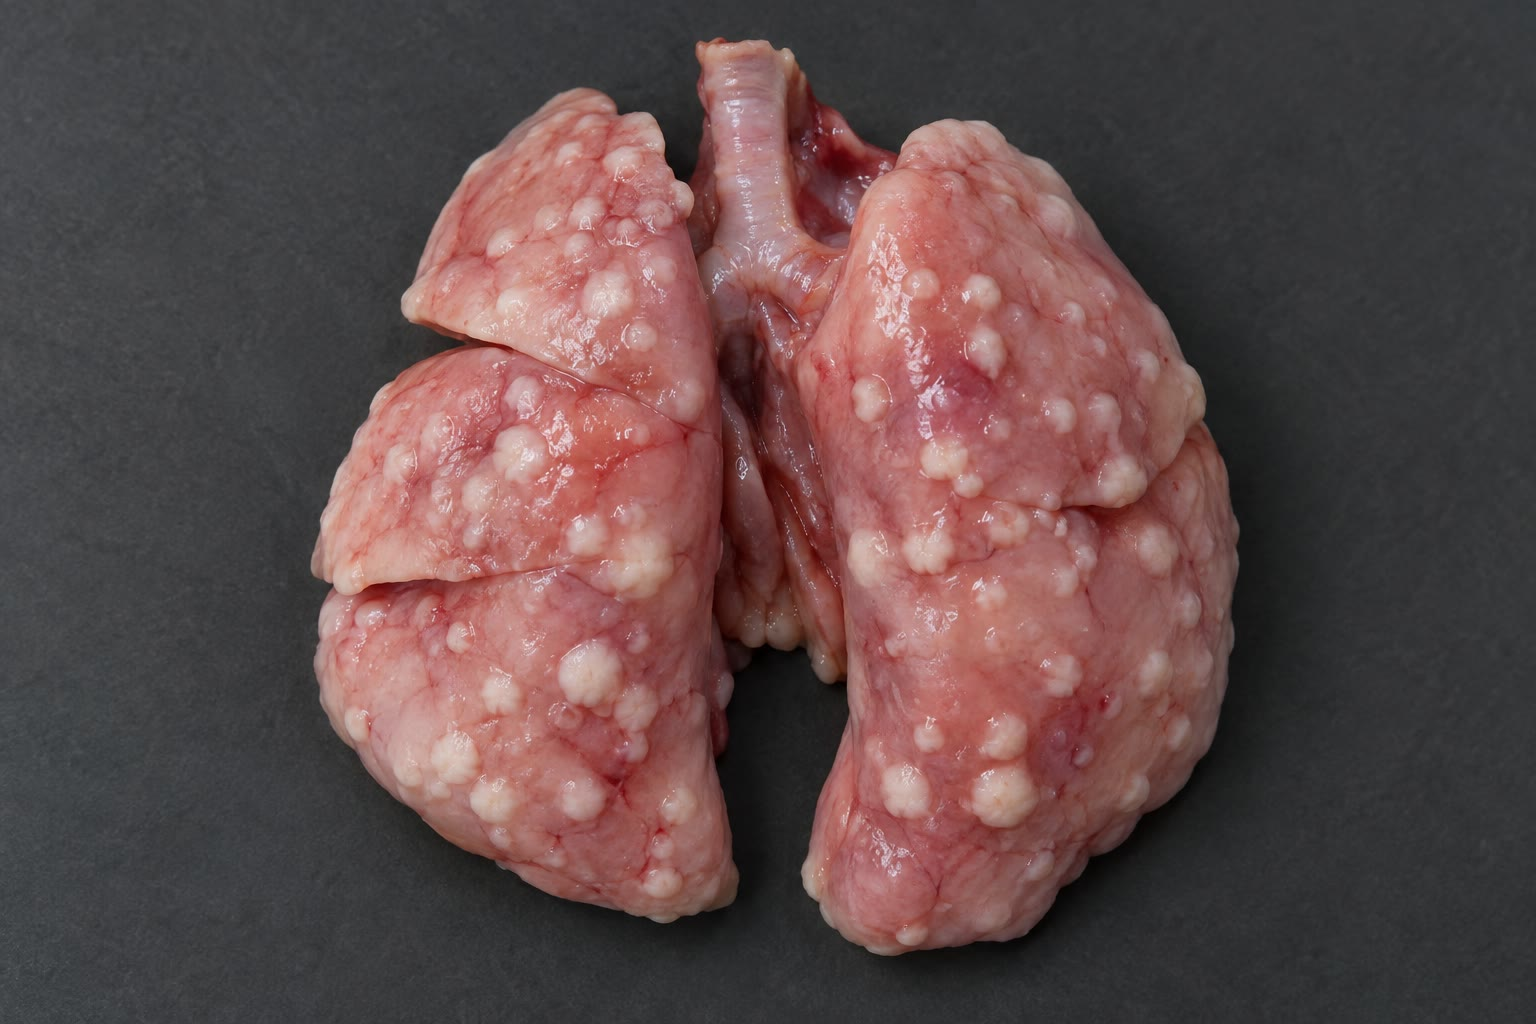
\includegraphics[width=0.54\linewidth]{images/book5/ai/b5-11-metastasis-lung.jpg}

{\small Kiri: sebuah sferoid \omterm{def:b3:cancer-biology:hallmarks}{tumor} (hijau) yang merekrut pembuluh baru (merah)
dari jejaring tetangganya --- yakni angiogenesis di dalam biakan. Kanan:
paru-paru mencit yang bertaburan \omterm{def:b3:cancer-biology:hallmarks}{metastasis}, dan tiap koloninya didirikan satu
sel yang selamat dari perjalanan lewat darahnya.}
\end{omfigure}

\begin{definition}[Invasi dan metastasis]\label{def:b3:cancer-biology:metastasis}
\index{invasi}\index{peralihan epitelium--mesenkim}\index{benih dan tanah}
Untuk bermetastasis, sebuah sel karsinoma harus meninggalkan epiteliumnya ---
kehilangan sambungan sel dan kekutubannya lalu memperoleh kemampuan bergerak,
yakni sebuah \emph{peralihan epitelium--mesenkim} yang digerakkan faktor
transkripsi yang biasanya dipakai dalam perkembangan embrio --- menguraikan
membran dasar dan matriksnya dengan protease yang disekresikannya, menyeberangi
dinding sebuah pembuluh darah atau limfa, bertahan hidup di dalam
peredarannya (kurang dari satu dari sepuluh ribu berhasil, karena dibunuh
gaya geser, ketiadaan pelekatan, dan sel pembunuh alami), tersangkut pada
sebuah alas kapiler organ lain, menyeberang keluar, lalu tumbuh di situ. Tempat
ia tumbuh tidaklah acak: \omterm{def:b3:cancer-biology:hallmarks}{kanker} payudara menuju tulang, paru-paru, hati, dan
otak, \omterm{def:b3:cancer-biology:hallmarks}{kanker} usus besar menuju hati, \omterm{def:b3:cancer-biology:hallmarks}{kanker} prostat menuju tulang --- yakni
\emph{benih dan tanah} Paget tahun 1889, yang sebagian dijelaskan aliran
darahnya dan sebagian oleh kecocokan antara selnya dan isyarat jaringannya.
Sebuah sel yang tersebar dapat tertidur bertahun-tahun sebelum tumbuh, dan
itulah sebabnya \omterm{def:b3:cancer-biology:hallmarks}{kanker} kambuh sedasawarsa sesudah tampak sembuh. \omterm{def:b3:cancer-biology:hallmarks}{Metastasis}
menyebabkan sembilan dari sepuluh kematian akibat \omterm{def:b3:cancer-biology:hallmarks}{tumor} padat, dan langkah
itulah yang paling sedikit dipahami.
\end{definition}

\begin{proposition}[Mengelak dari sistem kekebalan]\label{prop:b3:cancer-biology:immune}
\index{pengelakan kekebalan}\index{penghambat titik periksa}\index{neoantigen}
Mutasi sebuah \omterm{def:b3:cancer-biology:hallmarks}{tumor} menciptakan \emph{neoantigen}, yakni peptida yang tak
disajikan sel normal mana pun, dan sel~T sitotoksik mengenali lalu membunuh sel
\omterm{def:b3:cancer-biology:hallmarks}{tumor} --- itulah sebabnya pasien yang tertekan kekebalannya lebih banyak
mengidap \omterm{def:b3:cancer-biology:hallmarks}{kanker} dan sebabnya \omterm{def:b3:cancer-biology:hallmarks}{tumor} bermutasi banyak (melanoma, paru-paru, usus
besar yang \omterm{prop:b3:dna-repair:fidelity}{perbaikan salah pasangnya} cacat) paling baik menanggapi
imunoterapi. Sebuah \omterm{def:b3:cancer-biology:hallmarks}{tumor} yang tampak secara klinis adalah \omterm{def:b3:cancer-biology:hallmarks}{tumor} yang telah
lolos: dengan kehilangan molekul MHC yang menyajikan peptidanya, dengan
menyekresikan faktor penekan, dengan merekrut sel~T pengatur, dan yang
terutama dengan mengekspresikan PD-L1, yang menggarap reseptor penghambat PD-1
pada sel~T lalu mematikannya, yakni rem yang sama yang biasanya mengakhiri
sebuah tanggapan kekebalan (\cref{ch:b3:adaptive-immunity}). Antibodi yang
menghalangi PD-1 atau PD-L1, atau rem yang lebih awal yaitu CTLA-4, melepaskan
sel~T-nya; pada sebagian pasien --- seperlima sampai separuh bergantung pada
\omterm{def:b3:cancer-biology:hallmarks}{tumornya} --- antibodi itu menghasilkan remisi yang bertahan lama pada \omterm{def:b3:cancer-biology:hallmarks}{kanker}
yang dahulu tak terobati, dan efek sampingnya adalah autoimunitas, yakni
fungsi lain rem itu.
\end{proposition}

\section{Penyebab dan pengobatan}

\begin{proposition}[Penyebabnya]\label{prop:b3:cancer-biology:causes}
\index{karsinogen}\index{virus onkogenik}
\omterm{def:b3:cancer-biology:hallmarks}{Kanker} disebabkan apa pun yang menaikkan laju peristiwa pada
teoremanya atau menaikkan cacah sel yang berisiko. \emph{Karsinogen kimia},
yang sebagian besar menjadi mutagen sesudah diaktifkan hati: tujuh puluh
karsinogen asap tembakau, yang menyebabkan sepertiga kematian \omterm{def:b3:cancer-biology:hallmarks}{kanker} dan
menaikkan risiko \omterm{def:b3:cancer-biology:hallmarks}{kanker} paru-paru lima belas sampai dua puluh lima kali lipat;
aflatoksin dari biji-bijian berjamur; asbes, yang bukan mutagen melainkan
pengiritasi menahun. \emph{Radiasi}: cahaya ultraungu bagi kulit (dimer
\cref{ch:b3:dna-repair}), radiasi pengion bagi leukemia, tiroid,
dan payudara. \emph{Infeksi}, yakni seperenam \omterm{def:b3:cancer-biology:hallmarks}{kanker} sedunia: virus
papiloma, yang protein E6 dan E7-nya memusnahkan \omterm{def:b3:cancer-biology:genes}{p53} serta melumpuhkan
Rb lalu menyebabkan hampir seluruh \omterm{def:b3:cancer-biology:hallmarks}{kanker} serviks (sebuah vaksin kini
mencegahnya); virus hepatitis B dan C pada \omterm{def:b3:cancer-biology:hallmarks}{kanker} hati; virus Epstein--Barr
pada limfoma; \emph{Helicobacter pylori} pada \omterm{def:b3:cancer-biology:hallmarks}{kanker} lambung, lewat
peradangan yang berdasawarsa. \emph{Mutasi warisan} pada sebuah penekan
\omterm{def:b3:cancer-biology:hallmarks}{tumor}, yakni pukulan pertama saat lahir, pada sekitar \qty{5}{\%} \omterm{def:b3:cancer-biology:hallmarks}{kanker}. Dan
kebetulan: sebagian besar mutasi di dalam sebuah \omterm{def:b3:cancer-biology:hallmarks}{tumor} timbul dari galat biasa
replikasinya, sehingga jaringan yang paling banyak membelah --- usus besar,
kulit, darah --- paling banyak berkanker, dan risikonya naik dengan umur apa
pun yang dikerjakan orang.
\end{proposition}

\begin{theorem}[Mengapa satu obat gagal dan dua mungkin tidak]\label{thm:b3:cancer-biology:goldie-coldman}
\index{model Goldie--Coldman}\index{kekebalan obat}\index{terapi gabungan}
Misalkan sebuah \omterm{def:b3:cancer-biology:hallmarks}{tumor} berisi $N$ sel telah dihasilkan lewat pembelahan
berturut-turut dari satu sel, dan misalkan sebuah mutasi yang memberi kekebalan
terhadap sebuah obat tertentu timbul dengan laju $\mu$ tiap pembelahan sel.
Maka peluang bahwa \omterm{def:b3:cancer-biology:hallmarks}{tumornya} \emph{tidak} memuat sel yang kebal ketika
pengobatannya dimulai kira-kira
\[
P_{0} \approx e^{-\mu N},
\]
sehingga untuk $\mu N \gg 1$ kekebalannya sudah ada sebelumnya dengan
kepastian yang nyaris penuh. Bagi dua obat dengan mekanisme kekebalan yang
saling bebas, sebuah sel yang kebal terhadap keduanya timbul dengan laju
kira-kira $\mu_{1}\mu_{2}$ tiap pembelahan, dan $P_{0}
\approx e^{-\mu_{1}\mu_{2}N}$: dengan $N = 10^{9}$ dan $\mu = 10^{-7}$,
satu obat menghadapi $\mu N = 100$ klon kebal rata-rata, sedangkan dua obat
menghadapi peluang $10^{-5}$ bahwa satu saja sel kebal ganda ada.
\end{theorem}
\begin{proof}[Bukti sebagian]
Tumbuh dari $1$ menjadi $N$ sel memakan kira-kira $N$ pembelahan seluruhnya
(sebuah pohon berdaun $N$ memiliki $N - 1$ simpul dalam). Bila sebuah sel
kebal dihasilkan pada tiap pembelahan dengan peluang $\mu$ dan, sebagai
hampiran pertama, keturunannya tidak mati maupun mengalahkan sisanya, cacah
peristiwa kekebalannya bersebaran Poisson dengan rata-rata $\mu N$, dan
peluang tak satu pun adalah $e^{-\mu N}$. Mekanisme yang saling bebas
mengalikan peluang tiap pembelahannya. Hampirannya mengabaikan bahwa mutan
yang awal meninggalkan klon kebal yang lebih besar --- sebaran penuhnya adalah
sebaran Luria dan Delbrück, yang dibahas pada jilid Tahun~2 --- tetapi
peluang \emph{tak ada} mutan, yang menentukan apakah \omterm{def:b3:cancer-biology:hallmarks}{tumornya} dapat
disembuhkan, persis suku Poissonnya.
\end{proof}

\begin{example}[Terapi dan logikanya]\label{ex:b3:cancer-biology:therapy}
Pembedahan dan radioterapi menyingkirkan atau membunuh \omterm{def:b3:cancer-biology:hallmarks}{tumor} yang setempat;
radiasi membunuh lewat \omterm{def:b3:dna-repair:lesions}{putus untai ganda}, dan pemenggalannya menjadi dosis
harian membiarkan jaringan normal memperbaiki diri di antaranya
(\cref{ch:b3:dna-repair}). Kemoterapi sitotoksik --- zat pengalkil,
antimetabolit, racun \omterm{def:b3:cytoskeleton-motility:filaments}{mikrotubulus}, penghambat topoisomerase --- membunuh sel
yang membelah dari macam apa pun, dengan sel \omterm{def:b3:cancer-biology:hallmarks}{tumornya} sedikit lebih banyak,
lalu mengikuti hukum \emph{pembunuhan logaritmik}: tiap penggalnya membunuh
bagian yang tetap, katakanlah \qty{99}{\%}, sehingga enam penggal menciutkan
$10^{12}$ sel menjadi satu, dan enam penggal yang sama dibutuhkan entah
\omterm{def:b3:cancer-biology:hallmarks}{tumornya} besar entah kecil; rambut, usus, dan sumsum pasiennya, yang juga
membelah, menetapkan dosisnya. Terapi bersasaran menyerang sebuah cacat yang
menjadi tumpuan \omterm{def:b3:cancer-biology:hallmarks}{tumornya}: imatinib menghalangi kinase BCR--ABL lalu mengubah
leukemia mieloid menahun dari penyakit yang mematikan menjadi penyakit yang
menahun; trastuzumab mengikat HER2; penghambat PARP, penghambat Cdk4/6, dan
venetoklaks pada bab sebelumnya masing-masing memanfaatkan satu cacat.
Imunoterapi melepaskan sel~T-nya. Dan teoremanya mengatakan bagaimana semuanya
harus dipakai: dalam gabungan, sejak dini, ketika $N$ paling kecil --- dan
itulah yang dikerjakan kemoterapi ajuvan sesudah pembedahan --- serta dengan
obat yang mekanisme kekebalannya tak bertindihan. \omterm{def:b3:cancer-biology:hallmarks}{Tumornya} adalah populasi
yang berevolusi, dan pengobatan adalah seleksi.
\end{example}

\begin{omfigure}
\begin{tikzpicture}
\begin{axis}[
  width=0.7\linewidth, height=5.6cm,
  axis x line=bottom, axis y line=left,
  xmin=0, xmax=8, ymin=1, ymax=1e13, ymode=log,
  xlabel={penggal kemoterapi}, ylabel={sel tumor},
  xlabel style={font=\small, at={(axis description cs:0.5,-0.12)}, anchor=north},
  ylabel style={font=\small},
  tick label style={font=\small}, xtick={0,2,4,6,8},
  clip=false,
]
\addplot[very thick, omDef, mark=*, mark size=1.2pt] coordinates {(0,1e12) (1,1e10) (2,1e8) (3,1e6) (4,1e4) (5,1e2) (6,1)};
\addplot[very thick, omThm, mark=*, mark size=1.2pt] coordinates {(0,1e12) (1,1.01e10) (2,1.02e8) (3,1.04e6) (4,1.1e4) (5,200) (6,300) (7,600) (8,1200)};
\addplot[dashed, gray, domain=0:8, samples=2] {1e9};
\node[font=\scriptsize, gray, anchor=south west] at (axis cs:0.2,1.3e9) {terdeteksi, $10^{9}$};
\node[font=\scriptsize, omDef, anchor=south west] at (axis cs:0.3,1e4) {pembunuhan \qty{99}{\%} tiap penggal};
\node[font=\scriptsize, omThm, anchor=south west] at (axis cs:5.2,3e3) {satu sel kebal pada awalnya: kambuh};
\end{axis}
\end{tikzpicture}

{\small Hukum pembunuhan logaritmiknya. Tiap penggalnya membunuh bagian sel
yang sama, sehingga \omterm{def:b3:cancer-biology:hallmarks}{tumornya} menciut sebanyak beberapa dasawarsa tetap tiap
penggal lalu tak terdeteksi jauh sebelum ia lenyap (biru); satu sel kebal yang
telah ada sebelumnya bertahan pada tiap penggal lalu tumbuh kembali (merah).}
\end{omfigure}

\begin{remark}[Apa yang telah berubah]\label{rem:b3:cancer-biology:changed}
Separuh pasien yang didiagnosis \omterm{def:b3:cancer-biology:hallmarks}{kanker} di sebuah negara kaya kini
bertahan sepuluh tahun, berbanding seperempat pada tahun 1970. Kemajuannya
datang dari pencegahan (tembakau, vaksin hepatitis dan virus papiloma,
penapisan polip dan lesi serviks), dari deteksi yang lebih awal, dan dari
pengobatan yang menyusul dari biologi bab ini --- kemoterapi gabungan yang
menyembuhkan sebagian besar leukemia anak dan \omterm{def:b3:cancer-biology:hallmarks}{kanker} buah zakar, obat
bersasaran, serta imunoterapinya. Yang belum berubah adalah penyakit yang
telah bermetastasis, yang biologinya menjelaskannya tetapi belum
menyembuhkannya; kemajuan berikutnya akan datang dari memperlakukan \omterm{def:b3:cancer-biology:hallmarks}{tumor}
sebagai apa adanya, yakni populasi yang berevolusi di bawah seleksi yang
dipaksakan pengobatannya.
\end{remark}

\section{Latihan}

\begin{exercise}[$\star$]\label{exo:b3:cancer-biology:1}
Bedakanlah sebuah \omterm{def:b3:cancer-biology:genes}{onkogen} dari sebuah \omterm{def:b3:cancer-biology:genes}{gen penekan tumor} menurut mekanismenya,
menurut cacah alel yang harus berubah, dan dengan dua contoh masing-masing.
\end{exercise}

\begin{exercise}[$\star$]\label{exo:b3:cancer-biology:2}
Sebutkanlah \omterm{def:b3:cancer-biology:hallmarks}{ciri khas kanker} dan, bagi masing-masing, sebutkanlah satu gen bab
ini atau bab sebelumnya yang perubahannya memberikan ciri itu.
\end{exercise}

\begin{exercise}[$\star$]\label{exo:b3:cancer-biology:3}
Apa yang diamati Knudson tentang retinoblastoma turunan dan sporadis,
dan apa yang disimpulkannya?
\end{exercise}

\begin{exercise}[$\star$]\label{exo:b3:cancer-biology:4}
Jelaskanlah \omterm{met:b3:cancer-biology:ames}{uji Ames} dan mengapa ekstrak hati ditambahkan.
\end{exercise}

\begin{exercise}[$\star\star$]\label{exo:b3:cancer-biology:5}
Insidensi sebuah \omterm{def:b3:cancer-biology:hallmarks}{kanker} adalah $2\times 10^{-5}$ tiap tahun pada umur $40$
dan $2\times 10^{-3}$ pada umur $80$. Taksirlah eksponen hukum pangkat umurnya
dan cacah peristiwa pembatas laju yang disarankannya.
\end{exercise}

\begin{exercise}[$\star\star$]\label{exo:b3:cancer-biology:6}
Dengan \cref{prop:b3:cancer-biology:oxygen} dan $D =
\qty{2e-9}{m^2/s}$ serta $c_{0} = \qty{0.05}{mol/m^3}$, hitunglah $L$ bagi
jaringan yang memakai \qty{0.01}{mol/m^3/s} dan bagi sebuah \omterm{def:b3:cancer-biology:hallmarks}{tumor} yang memakai
tiga kali lipatnya. Mengapa \omterm{def:b3:cancer-biology:hallmarks}{tumor} yang tumbuh cepat menjadi nekrotik lebih awal?
\end{exercise}

\begin{exercise}[$\star\star$]\label{exo:b3:cancer-biology:7}
Sebuah \omterm{def:b3:cancer-biology:hallmarks}{tumor} berisi $10^{11}$ sel diobati dengan obat yang membunuh
\qty{99.9}{\%} tiap penggal. Berapa penggal untuk menciutkannya di bawah satu
sel? Mengapa \omterm{def:b3:cancer-biology:hallmarks}{tumornya} tak terdeteksi sesudah dua penggal padahal
$10^{5}$ sel tersisa, dan apa yang tersirat dari hal itu bagi penghentian
pengobatannya?
\end{exercise}

\begin{exercise}[$\star\star$]\label{exo:b3:cancer-biology:8}
Jelaskanlah mengapa sebuah mutasi pada EGFR dan sebuah mutasi pada KRAS jarang
ditemukan pada \omterm{def:b3:cancer-biology:hallmarks}{tumor} paru-paru yang sama, dan mengapa sebuah \omterm{def:b3:cancer-biology:hallmarks}{tumor} yang diobati
penghambat EGFR kerap kambuh dengan sebuah mutasi KRAS.
\end{exercise}

\begin{exercise}[$\star\star$]\label{exo:b3:cancer-biology:9}
Protein E6 dan E7 virus papiloma melumpuhkan \omterm{def:b3:cancer-biology:genes}{p53} dan Rb. Jelaskanlah
bagaimana hal itu menggerakkan \omterm{def:b3:cancer-biology:hallmarks}{kanker} serviks, mengapa hal itu memakan
beberapa dasawarsa, dan mengapa sebuah vaksin yang diberikan sebelum aktivitas
seksual mencegahnya.
\end{exercise}

\begin{exercise}[$\star\star\star$]\label{exo:b3:cancer-biology:10}
Perluaslah argumen Armitage--Doll agar tiap pukulan dapat mengembangkan
klonnya sebesar faktor $g$ sebelum pukulan berikutnya: tunjukkanlah bahwa
insidensinya berpangkat $t$ yang sama tetapi prafaktornya dikali $g^{k-1}$,
lalu bahaslah mengapa $k$ yang dicocokkan dari sebuah kurva umur menjadi batas
atas cacah pemacunya.
\end{exercise}

\begin{exercise}[$\star\star\star$]\label{exo:b3:cancer-biology:11}
Dengan \cref{thm:b3:cancer-biology:goldie-coldman}, bandingkanlah (a)
pengobatan sebuah \omterm{def:b3:cancer-biology:hallmarks}{tumor} berisi $10^{9}$ sel dengan obat A selama enam penggal
lalu obat B selama enam penggal, dan (b) pemberian A dan B bersama sejak awal,
ketika $\mu_{A} =
\mu_{B} = 10^{-7}$. Hitunglah $P_{0}$ bagi tiap siasatnya lalu jelaskan
mengapa gabungan yang dini menjadi kelaziman.
\end{exercise}

\begin{exercise}[$\star\star\star$]\label{exo:b3:cancer-biology:12}
Paradoks Peto: seekor gajah memiliki sel seratus kali lebih banyak daripada
manusia dan hidup sama lamanya, namun tidak lebih banyak berkanker. Dengan
teorema bab ini, katakanlah apa harapan naifnya, lalu usulkanlah dua
mekanisme yang dengannya hewan besar dapat memecahkan masalah itu (gajah
memiliki dua puluh salinan \emph{TP53}).
\end{exercise}

\section{Soal: Aritmetika Sebuah Tumor}

\begin{problem}[{Soal akhir pekan --- sebuah tumor yang tumbuh dari satu sel
lalu ditakar sampai terdeteksi, kurva umurnya yang dibaca untuk mencari cacah
pukulannya, pasokan oksigen serta inti nekrotiknya yang dihitung, dan
pengobatannya yang direncanakan melawan kepastian kekebalan, berakhir pada
tahun sampai terdeteksi, kedalaman tumor yang hidup di sekeliling sebuah
pembuluh, serta peluang bahwa sebuah gabungan menyembuhkan}]
\label{pb:b3:cancer-biology:1}
Data: sebuah sel \omterm{def:b3:cancer-biology:hallmarks}{tumor} bervolume \qty{1000}{\micro m^3}; waktu
pelipatduaannya \qty{100}{d}; terdeteksi pada \qty{1}{cm^3}; muatan mematikan
\qty{1}{kg}. Kurva umurnya: insidensi $1\times 10^{-5}$ tiap tahun pada umur
$30$ dan $3\times
10^{-3}$ pada umur $80$. Oksigennya: $D = \qty{2e-9}{m^2/s}$, $c_{0} =
\qty{0.05}{mol/m^3}$, $q = \qty{0.03}{mol/m^3/s}$ di dalam \omterm{def:b3:cancer-biology:hallmarks}{tumornya};
kapiler di dalam \omterm{def:b3:cancer-biology:hallmarks}{tumor} yang berpembuluh berjarak \qty{150}{\micro m}. Terapinya:
tiap penggal membunuh \qty{99}{\%}; laju mutasi kekebalannya $10^{-7}$ tiap
pembelahan tiap obat; satu penggal tiap tiga minggu; \omterm{def:b3:cancer-biology:hallmarks}{tumornya} tumbuh kembali
di antara penggalnya dengan waktu pelipatduaan yang sama.

\medskip
\noindent\textbf{Bagian I --- Pertumbuhan.}
\begin{enumerate}
  \item Berapa sel di dalam \qty{1}{cm^3}? Berapa pelipatduaan dari satu
        sel?
  \item Berapa tahun dari sel pendirinya sampai terdeteksi?
  \item Berapa pelipatduaan, dan berapa tahun, dari terdeteksi sampai
        muatan mematikannya? Bandingkanlah kedua selangnya.
  \item Banyak \omterm{def:b3:cancer-biology:hallmarks}{tumor} terdeteksi pada \qty{1}{cm^3} tetapi baru tumbuh
        selama lima tahun. Apa yang pasti benar tentang waktu pelipatduaannya
        pada masa awalnya, atau tentang hukum pertumbuhannya?
  \item Hanya bagian $f$ sel di dalam sebuah \omterm{def:b3:cancer-biology:hallmarks}{tumor} yang membelah pada tiap
        saat (yakni bagian yang tumbuh), dan sebagian mati. Bila selnya
        berdaur dalam \qty{2}{d} tetapi \omterm{def:b3:cancer-biology:hallmarks}{tumornya} berlipat dua dalam $100$
        hari, apa yang dikatakan hal itu tentang imbangan kelahiran dan
        kematiannya?
  \item Mengapa kemoterapi pembunuhan logaritmik yang sama lebih mengampuni
        \omterm{def:b3:cancer-biology:hallmarks}{tumor} yang tumbuh lambat daripada yang cepat, namun yang cepat itu
        tumbuh kembali lebih cepat di antara penggalnya?
\end{enumerate}

\medskip
\noindent\textbf{Bagian II --- Pukulan.}
\begin{enumerate}[resume]
  \item Dari kedua insidensinya, hitunglah eksponen $k - 1$ kurva
        umurnya dan cacah peristiwa $k$ yang tersirat.
  \item Bila tiap peristiwanya terjadi pada $u = 10^{-6}$ tiap sel tiap tahun
        di dalam $N = 10^{8}$ sel yang rentan, apa yang diramalkan teoremanya
        bagi risiko kumulatif pada umur $70$ dengan $k$ Anda? Apakah masuk
        akal? Apa yang kurang?
  \item Ulangilah dengan pengembangan klonal sebesar faktor $g = 100$ sesudah
        tiap dari $k - 1$ pukulan pertamanya, memakai
        \cref{exo:b3:cancer-biology:10}.
  \item Seorang pembawa mewarisi satu pukulan. Dengan faktor berapa
        insidensinya pada umur $40$ dinaikkan, bila laju yang lain tak
        berubah? (Bandingkanlah $(ut)^{k-1}$ dengan $(ut)^{k}$ pada $t = 40$.)
  \item Merokok mengalikan $u$ bagi salah satu peristiwanya dengan $10$.
        Dengan faktor berapa insidensinya naik bila peristiwa itu satu dari
        $k$; bila peristiwa itu dua di antaranya?
  \item Jelaskanlah mengapa berhenti merokok pada umur lima puluh menurunkan
        risiko \omterm{def:b3:cancer-biology:hallmarks}{kanker} paru-paru di bawah risiko perokok yang melanjutkan,
        tetapi tak pernah sampai ke risiko orang yang tak pernah merokok.
\end{enumerate}

\medskip
\noindent\textbf{Bagian III --- Pasokan.}
\begin{enumerate}[resume]
  \item Hitunglah kedalaman penembusan oksigen $L$ di dalam \omterm{def:b3:cancer-biology:hallmarks}{tumornya}.
  \item Sebuah sferoid tanpa pembuluh: berapa garis tengah maksimum ketika
        setiap selnya masih beroksigen? Berapa tebal tepi yang hidup
        sebuah sferoid \qty{2}{mm}, dan berapa bagian volumenya
        yang hidup?
  \item Di dalam sebuah \omterm{def:b3:cancer-biology:hallmarks}{tumor} berpembuluh dengan kapiler berjarak
        \qty{150}{\micro m}, apakah setiap selnya beroksigen? Sel yang mana
        yang hipoksia, dan mengapa hal itu berarti bagi radioterapi (oksigen
        memakukan kerusakan radiasinya) dan bagi seleksi sel yang \omterm{def:b3:cancer-biology:genes}{p53-nya} mutan?
  \item Sebuah obat memparuhkan kerapatan kapiler \omterm{def:b3:cancer-biology:hallmarks}{tumornya}. Hitunglah ulang
        jaraknya lalu katakan apa yang terjadi pada sel yang berada di tengah
        antara pembuluhnya.
  \item Sel hipoksianya beralih ke glikolisis, sehingga membuat \qty{2}{ATP}
        tiap glukosa alih-alih $30$. Dengan faktor berapa sel itu harus
        menaikkan penyerapan glukosanya agar pasokan ATP-nya terjaga, dan
        bagaimana hal itu dimanfaatkan dalam pencitraan \omterm{def:b3:cancer-biology:hallmarks}{tumor}?
  \item Jelaskanlah mengapa terapi antiangiogenesis sendirian jarang
        menyembuhkan tetapi dapat membantu kemoterapi mencapai \omterm{def:b3:cancer-biology:hallmarks}{tumornya}.
\end{enumerate}

\medskip
\noindent\textbf{Bagian IV --- Pengobatan.}
\begin{enumerate}[resume]
  \item Sebuah \omterm{def:b3:cancer-biology:hallmarks}{tumor} \qty{1}{cm^3} diobati dengan satu obat. Berapa
        penggal yang menciutkannya di bawah satu sel, dengan mengabaikan
        pertumbuhan kembali dan kekebalannya?
  \item Di antara penggalnya (tiga minggu) penyintasnya tumbuh kembali. Dengan
        faktor berapa? Hitunglah ulang pembunuhan netonya tiap daur dan cacah
        daur yang dibutuhkan.
  \item Hitunglah harapan cacah sel yang kebal terhadap obatnya pada
        awal pengobatannya dan peluang bahwa tak ada satu pun.
  \item Dua obat dengan mekanisme yang saling bebas diberikan bersama.
        Berapa peluang bahwa tak ada sel kebal ganda pada awalnya?
        Pada \omterm{def:b3:cancer-biology:hallmarks}{tumor} berisi $10^{12}$ sel?
  \item Terapi ajuvan diberikan sesudah pembedahan, ketika barangkali $10^{6}$
        sel tersisa tak terdeteksi. Hitunglah ulang peluangnya bagi satu
        dan dua obat, lalu nyatakan pelajarannya.
  \item Sebuah imunoterapi mengimbas sel~T yang membunuh sel mana pun yang
        menyajikan sebuah neoantigen. Mengapa kekebalan terhadapnya menjadi
        masalah yang berbeda dari kekebalan terhadap penghambat kinase, dan
        \omterm{def:b3:cancer-biology:hallmarks}{tumor} yang mana yang disarankan teoremanya paling cocok baginya?
  \item Ringkaskanlah: tahun dari sel pendirinya sampai terdeteksi
        (pertanyaan~2), kedalaman \omterm{def:b3:cancer-biology:hallmarks}{tumor} yang hidup di sekeliling sebuah
        pembuluh (pertanyaan~13), dan peluang bahwa gabungan dua obatnya
        tak menghadapi satu pun sel kebal di dalam \omterm{def:b3:cancer-biology:hallmarks}{tumor} \qty{1}{cm^3}
        (pertanyaan~22).
\end{enumerate}
\end{problem}
